\section{Drogon The Robot Simulator}
{
    \subsection{Introduction}
    The name \textbf{Drogon} was inspired from an invincible and all rounder character from a famous novel by George. R. R. Martin cite???

    With the availability of a highly customizable modeling solution such as \texttt{Drogons}, I was tempted to modify it to be used with a robotic arm. This might seem like an over-estimation of the project requirements but, an often undervalued yet important step of project management is the optimum utilization of the available skill-set.

    Comprehensiveness is the core attribute of this simulator. It provides, under one screen, the flexibility to introduce an elementary change in the design, like, the maximum speed of an actuator and directly observe the consequences on all of the analysis tools. One can choose to programmatically or manually signal an actuator to move in a particular direction and position, and visualize the outcome in a $3$D preview window.

    Besides comprehensiveness, our design tool offers a set of powerful analysis tools which enabled us to solve complex robot maneuvers and optimize the solution. Performing mechanical simulation with simplified real world constraints, $3$D live preview of the moving robot, work-space optimizer, $2$D art drawing, investigating the actuator velocity in continuous and discrete demain are some of the tools we used for optimization in our design.

    The tool can easily integrate with Microcontrollers, Proteus and SolidEdge to give more design flexibility.
    \subsection{Simulation}
    The simulator section of \texttt{Drogon v2} considers the robot fixed on a horizontal surface at a point $(0, 0, 0)$ and allows the user to signal each actuator either manually or programmatically. These movements are then simulated in tiny timer intervals as linear variables (just like the other simulators). It should be noted that the simulator simulates only the kinematics of the manipulator yet. However, for the sake of simplicity, all the other parameters are not considered. For example, simplest of the motors is the DC stepper motor which is simulated in the current version. Still, one could modify the simulation thread routine to implement a PID controller as well. An example of which can be seen in the simulation of the $7$th force control actuator of the robot. Obviously, a price would have to be paid, namely; excessive computational load, software design complexity.

    More details on the working principles of the simulator will be discussed in later chapters. Also, the installation and usage of the tool is described in detail in Appendix B.

    \subsection{About the Tools}

    An shape independent model of the robot under simulation can be visualized in real time using ``$3D$ Animation'' tool as seen in Fig. \ref{Fig3D}. The ``Robot Feet Position'' tool gives a superior insight on the stability of the robot. It can be seen in Fig. 1A(e) that the center of gravity plot can help optimize the motion where stability is a concern. Using the trajectory of the center of the robot in the global frame of reference can help determine the most efficient actuator movements which can be used to displace the robot from a specific position. Screen shots of the plot produced using the ``Top Trajectory'' tool can be seen in Fig. 1A(d).


        \begin{figure}
          \centering
          \includegraphics[width=0.7\textwidth]{3D.png}
          \caption{A screenshot of the $3$D representation tool. The blue sphere under the end effector shows the target given to the robot.
          } \label{Fig3D}
        \end{figure}

    All of the tools can output in real time. The robot configuration and other parameters change with time, producing animations which make it easier to decipher the underlying information.

    \subsection{Workspace Optimization}
    The workspace optimizer allows to simulate the robot solution recursively through discrete sections of the defined workspace and evaluates the degrees of freedom the robot has  specific parts of the workspace. It then colors the segments to give a more clear idea of the robot workspace. The user can then modify the robot and see, in-result, the change in the workspace. A typical output of the workspace is show in Fig.

        \begin{figure}
          \centering
          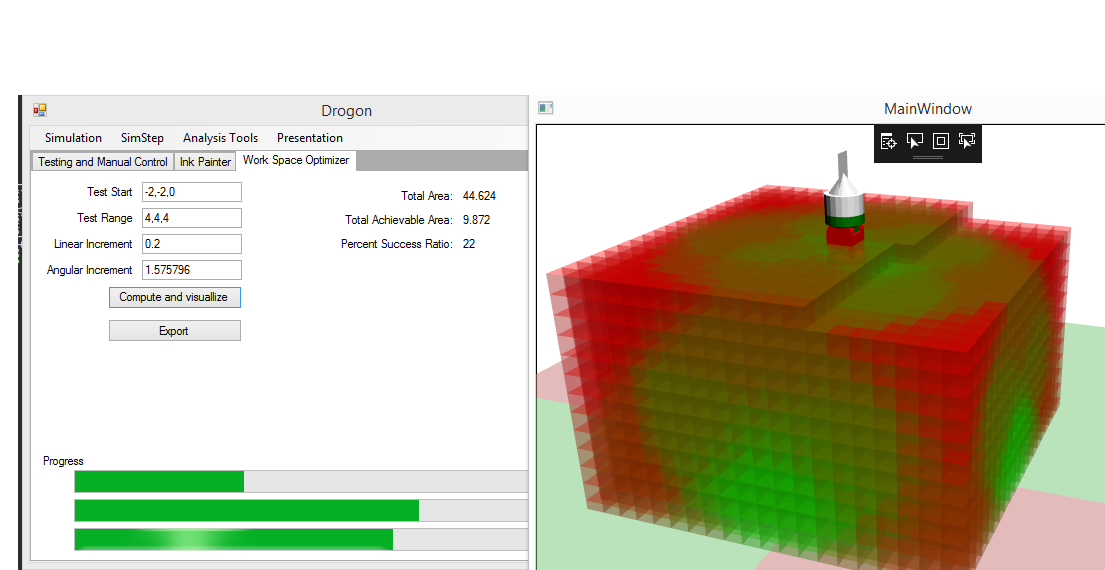
\includegraphics[width=0.9\textwidth]{WorkSpaceOptimer.png}
          \caption{The workspace is coded in colors. Purely green blocks represent a point where the robot has all of the degrees of freedom and the slightly red blocks indicate the parts where robot starts to loose one or more degrees of freedom.
          } \label{FigWorkspace}
        \end{figure}
    \subsection{Script Path Planner}
    As already mentioned, I've included a tool to construct bezier rotation splines in the tool which can serialize the data in computer files and also load from existing files. A screenshot can be seen in Fig.

        \begin{figure}
          \centering
          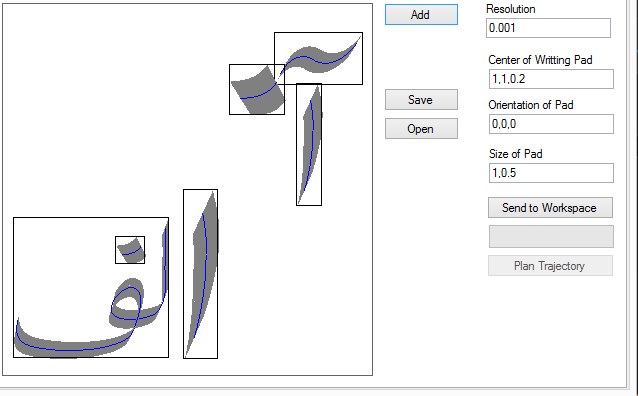
\includegraphics[width=0.9\textwidth]{SctiptEditor.png}
          \caption{The script maker can manage multiple splines and render robot trajectory according to the user resolution requirement.
          } \label{FigWorkspace}
        \end{figure}
    \subsection{Script Motion Simulator}
    Once the script is constructed using the script maker, it can be transported to the workspace in any orientation. The robot then plans how to make the required maneuvers and sibilates the behaviour. A screenshot of a robot writting a script can be seen in figure \ref{FigScriptMotion}
        \begin{figure}
          \centering
          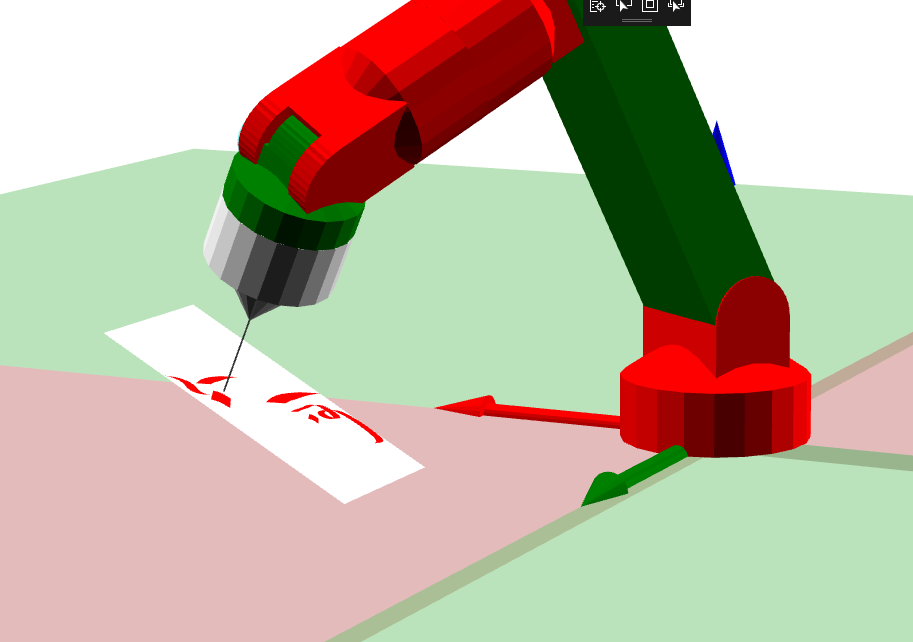
\includegraphics[width=0.9\textwidth]{writting.PNG}
          \caption{Robot writting on a slanted plane.
          } \label{FigScriptMotion}
        \end{figure}
}
\subsection{Requirements and Features}
\subsection{3D Visualizer}
\subsection{Workspace Optimizer}
\subsection{PID Tuner}
\subsection{Rotating Spline Importer}
\subsection{Usage}
\subsection{Interface}
\subsubsection{Manual Control}
\subsubsection{Analysis Tools}
\subsection{Development}
\subsubsection{Code Organization}
\subsubsection{The SphericalRobot Class}
\subsection{Simulation}
\subsubsection{Assumptions and Limitations}
\subsubsection{Accuracy of simulated Quantities}
\subsubsection{Forward Kinematics}
\subsubsection{Rotating Bezier Spline Curves}
\subsection{Sample Results}
\subsubsection{Accuracy}
\subsection{Areas that Need Improvement}
